\documentclass[14pt, a4paper]{article}

\usepackage[utf8]{inputenc}
\usepackage[T2A]{fontenc}

\usepackage{graphicx}
\graphicspath{ {images/} }

\title{ЛАБОРАТОРНАЯ РАБОТА №4
ПЕРЕХОДНЫЕ ПРОЦЕССЫ В НЕРАЗВЕТВЛЕННЫХ
ЭЛЕКТРИЧЕСКИХ ЦЕПЯХ
}
\author{Новоженов П.А. ЭН-26}
\date{}

\begin{document}

    \maketitle

    \thispagestyle{empty}

    \clearpage

    \section*{Цель работы}
        Экспериментальное исследование апериодических и колебательных
        переходных процессов в линейных электрических цепях первого и второго
        порядков и сопоставление экспериментальных результатов с предварительно
        рассчитанными параметрами.

        mkjndfjnd
        
    \section*{Задание 1. Определение постоянной времени}
        Рассчитаем переходный процесс в RL цепи.
        $$U = 4 \ V$$
        $$R = R_{kr} = 2\sqrt{\frac{L}{C}} = 200 \ \Omega$$
        $$L = 160\  mH$$
        $$C = 16 \ \mu F$$

        $$i(t) = \frac{U}{R} (1 - \exp(-\frac{t}{\tau})) = \frac{U}{R} (1 - \exp(-\frac{tR}{L}))$$
        $$u_L(t) = U\exp(-\frac{t}{\tau}) = U \exp(-\frac{tR}{L})$$
        $$\tau = \frac{L}{R} = 0.0008 \ c$$

        Получим такой график. Значения напряжения уменьшены в 200 раз.

        {
            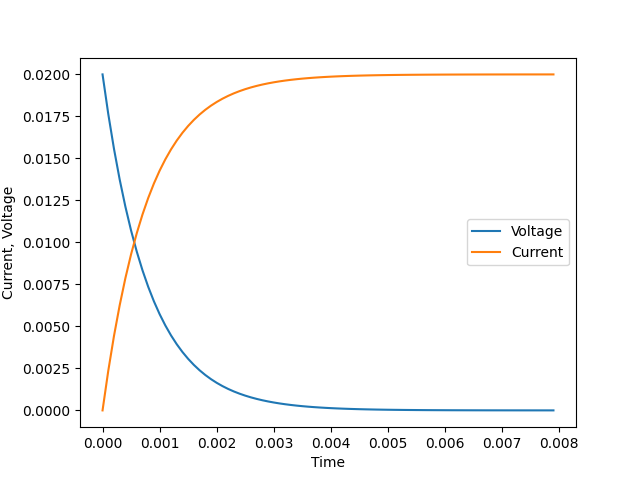
\includegraphics[width=0.8\textwidth]{plot_1.png}
            \centering
        }

        $$U(0) = 4 \ V$$
        $$U(\tau) = 1.47 \ V \ (\frac{U(0)}{e})$$
        $$U(2\tau) = 0.54 \ V \ (\frac{U(0)}{e^2})$$
        $$U(3\tau) = 0.20 \ V \ (\frac{U(0)}{e^3})$$

    
    \section*{Задание 2. Рассчет коэффициента затухания}
        $$U = 4 \ V$$
        $$R = 0.1R_{kr} = 2\sqrt{\frac{L}{C}} = 20 \ \Omega$$
        $$L = 160\  mH$$
        $$C = 16 \ \mu F$$

        $$\alpha = \frac{R}{2L} = \frac{}{} = 62.5$$
        $$\omega_o = \frac{1}{\sqrt{LC}} = 625$$
        $$\omega_c = \sqrt{\omega_o^2 - \alpha_2} = 621.8$$
        $$T_{c} = \frac{2\pi}{\omega_c} = 0.01 \ c$$

        $$i(t) = \frac{U}{\omega_c L}\cdot e^{-\alpha t}\sin(\omega_c t)$$

        {
            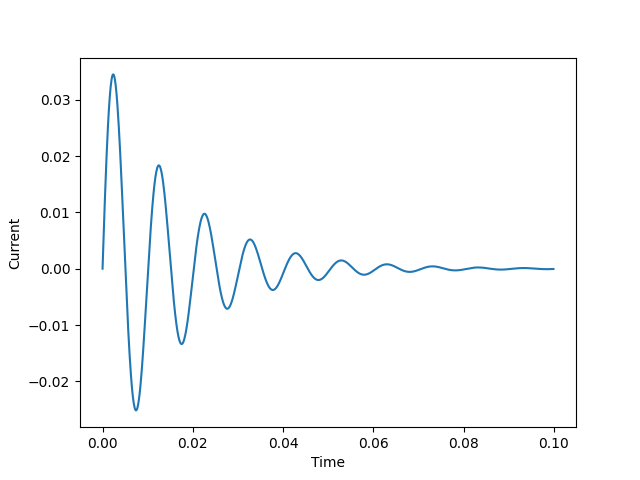
\includegraphics[width=0.8\textwidth]{plot_2.png}
            \centering
        }
    
    
    \section*{Задание 3. RL и RC-цепи}
        {
            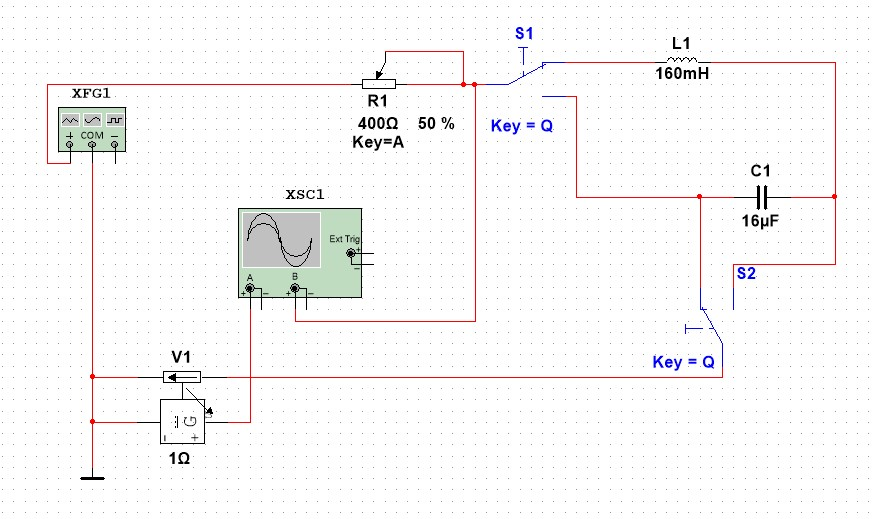
\includegraphics[width=0.8\textwidth]{Design.jpg}
            \centering
        }

        {
            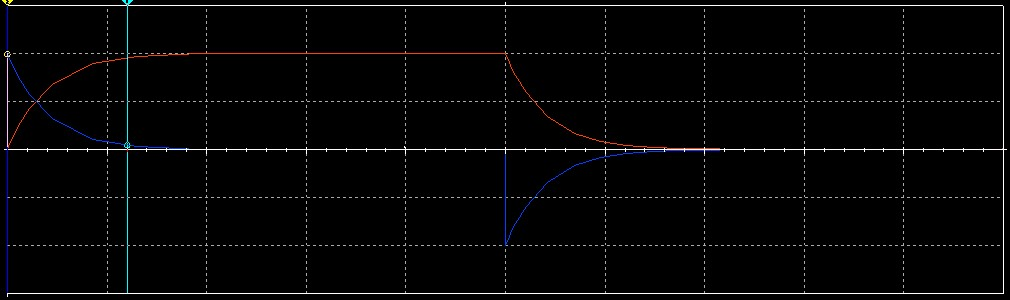
\includegraphics[width=0.8\textwidth]{OSC_RL.jpg}
        }

        Синий - напряжение, Красный - ток.

        $$\tau = 800 \mu s$$
        $$i(0) = 0.024 \ mA$$
        $$u(0) = 3.995 \ V$$
        $$i(\tau) = 12.7 \ mA$$
        $$u(\tau) = 1.460 \ V$$
        $$i(2\tau) = 17.3 \ mA$$
        $$u(2\tau) = 535.433 \ V$$
        $$i(3\tau) = 19.066 \ mA$$
        $$u(3\tau) = 0.186 \ V$$

        {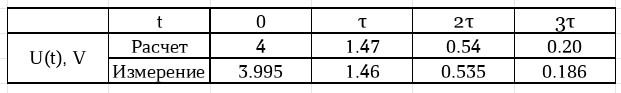
\includegraphics{table3.jpg}}

    
    \section*{Задание 4. RLC-цепь}

    {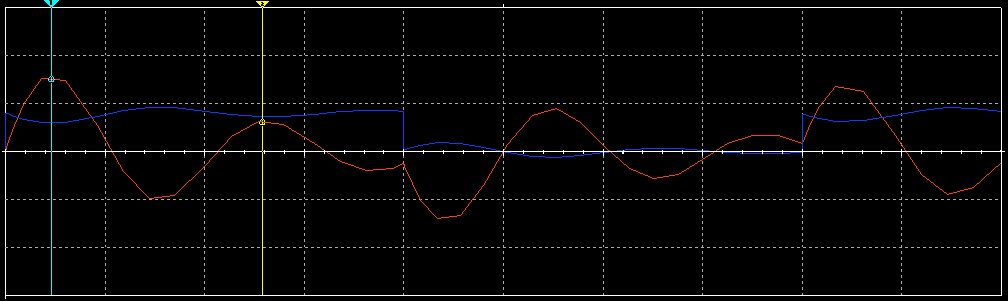
\includegraphics[width=1.2\textwidth]{OSC_RLС.jpg}}

    $$T_c = 10.592 \ ms$$
    $$I_1 = 30.048 \ mA; \ I_2 = 12.358 \ mA; \ I_1 - I_2 = 17.690 \ mA $$
    $$\alpha = \frac{\ln(\frac{I_1}{I_2})}{T_c} = 83.8 \ s^{-1}$$

    $$\omega_c = \frac{2\pi}{T_c} = 593.2$$




    \section*{Задание 5. Апериодический переходный процесс}
        Осцилограмма апериодичного процесса:

        {
                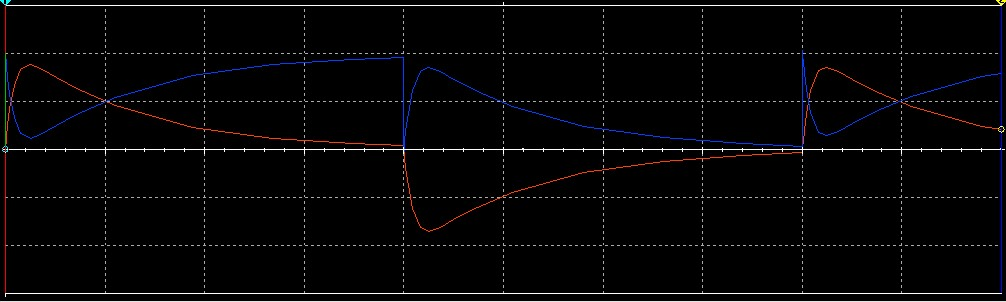
\includegraphics[width=1\textwidth]{OSC_Aperiod.jpg}
        }

        После уменьшения сопротивления в два раза:

        {
                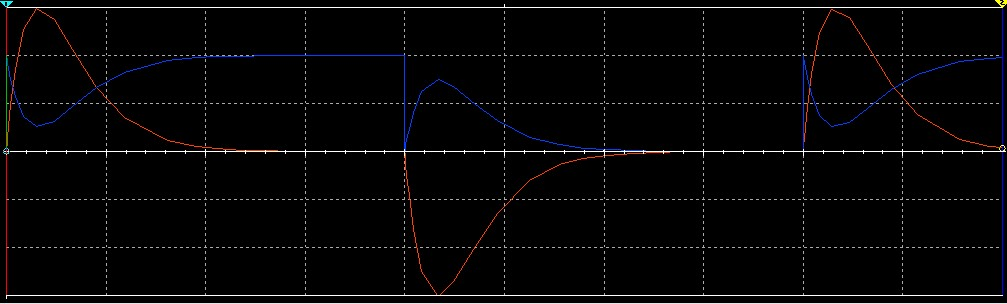
\includegraphics[width=1\textwidth]{OSC_Aperiod50.jpg}
        }

        С увеличением сопротивления уменьшается крутизна нарастания критического переходного тока и напряжения. 

    \section*{Вывод}

        В ходе данной лабораторной работы мы исследовали апериодические и колебательные 
        переходный процессы в линейных электрических цепях первого и второго
        порядков и провели сопоставление экспериментальных результатов с предварительно
        рассчитанными параметрами.


\end{document}